\documentclass[article]{uom-coursework}
% \usepackage[showframe]{geometry}

\usetikzlibrary{automata, positioning, arrows,
arrows.meta}

\usepackage{float}
\usepackage{syntax}
\usepackage[ruled]{algorithm2e}

% \usepackage{etoolbox}% http://ctan.org/pkg/etoolbox
% \makeatletter
% \patchcmd{\lst@GLI@}% <command>
%   {\def\lst@firstline{#1\relax}}% <search>
%   {\def\lst@firstline{#1\relax}\def\lst@firstnumber{#1\relax}}% <replace>
%   {\typeout{listings firstnumber=firstline}}% <success>
%   {\typeout{listings firstnumber not set}}% <failure>
% \makeatother

% \makeatletter
% \patchcmd{\lst@GLI@}% <command>
%   {\def\lst@firstline{#1\relax}}% <search>
%   {\def\lst@firstline{#1\relax}\def\lst@firstnumber{#1\relax}}% <replace>
%   {\typeout{listings firstnumber=firstline}}% <success>
%   {\typeout{listings firstnumber not set}}% <failure>
% \makeatother

% \tracingpatches
%
% \makeatletter
% \ifpatchable{\lst@GLI@}% <command>
%   {\def\lst@firstline{#1\relax}}% <search>
%     {
%         \patchcmd{\lst@GLI@}% <command>
%           {\def\lst@firstline{#1\relax}}% <search>
%           {\def\lst@firstline{#1\relax}\def\lst@firstnumber{#1\relax}}% <replace>
%           {\typeout{listings firstnumber=firstline}}% <success>
%           {\typeout{listings firstnumber not set}}% <failure>
%     }% <true>
%   {\typeout{listings firstline not set}}% <false>
% \makeatother

\counterwithout{section}{chapter}

\lstset{inputpath={../src}, language=C++}

\def\CC{{C\nolinebreak\raisebox{.25ex}{\scriptsize\bfseries{++}}}}

\newcommand{\listref}[1]{Listing~\ref{lst:#1}}
\newcommand{\figref}[1]{Figure~\ref{fig:#1}}

% Biblography
% \addbibresource{dsa.bib}

\title{Compiler Theory and Practice}
\tagline{Coursework}
\author{Juan Scerri}
\authorid{123456A}
\courseworkname{Some Degree}
\doctype{coursework}
\courseworkdate{\monthyeardate\today}
\subjectcode{CPS2000}


\begin{document}

%----------------------------------
%	Front Matter
%----------------------------------

\pagestyle{umpage}

\frontmatter

\maketitle % Print the title page

\tableofcontents % Print the table of contents

\clearpage

\lstlistoflistings

\clearpage

\mainmatter

\chapter*{Report}
\label{chap:report}
\addcontentsline{toc}{chapter}{\nameref{chap:report}}

\section{Lexer}

\subsection{Design \& Implementation}

The lexer was split into three-main components. A
DFSA class, a generic table-driven lexer, and a
lexer builder.

\subsubsection{The DFSA}

The DFSA class is an almost-faithful
implementation of the formal concept of a DFSA.
\listref{dfsadecl}, outlines the behaviour of the
DFSA. Additionally it contains a number of helper
functions which facilitate getting the initial
state and checking whether a state or a transition
category is valid. These helpers specifically,
\texttt{getInitialState()} is present since after
building the DFSA there is no guarantee the
initial state used by the user will be the same.

\lstinputlisting[
firstline=14,
lastline=44,
caption={DFSA Class Declaration (lexer/DFSA.hpp)},
label=lst:dfsadecl
]{lexer/DFSA.hpp}

The only significant difference is the
\texttt{getTransition()} functions. In fact, it
accepts a vector of transition categories instead
of a single category.

This is because a symbol e.g. `\texttt{a}',
`\texttt{9}' etc, might be valid for multiple
categories. For instance `\texttt{a}` is
considered to be both a letter and a number in
hexadecimal.

The DFSA for accepting the micro-syntax
\texttt{PArL} is built as follows.

Let $\mathfrak{U}$ be the set of all possible
characters under the system encoding (e.g. UTF-8).

The will use the following categories:

\begin{itemize}
    \item $L \coloneq \{
        \texttt{A},\ldots,\texttt{Z},\texttt{a},\ldots,\texttt{z}\}$
    \item $D \coloneq
        \{\texttt{0},\ldots,\texttt{9}\}$
    \item $H \coloneq
        \{\texttt{A},\ldots,\texttt{F},\texttt{a},\ldots,\texttt{f}\}
        \cup D$
    \item $S \coloneq \{\alpha \in \mathfrak{U}
        \colon \alpha\ \text{is
    whitespace}\}\setminus\{\texttt{LF}\}$
\end{itemize}

Note: \texttt{LF} refers to line-feed or as it is
more commonly known `\texttt{\textbackslash n}'
i.e. new-line.

Together these categories form our alphabet
$\Sigma$:

$$\Sigma \coloneq L \cup D \cup S \cup
\{\texttt{.},\texttt{\#},\texttt{\_},\texttt{(},\texttt{)},\texttt{[},\texttt{]},\texttt{\{},\texttt{\}},\texttt{*},\texttt{/},\texttt{+},\texttt{-},\texttt{<},\texttt{>},\texttt{=},\texttt{!},\texttt{,},\texttt{:},\texttt{;},\texttt{LF}\}$$

Now, the following drawing describe the
transitions of the DFSA. For improved readability
the DFSA has been split across mulitple drawings.
Hence, in each drawing  initial state $0$ refers
to the \emph{same} initial state (a DFSA has one
and only one initial state).

Additionally, each final state is annotated with
the token type it should produce.

\tikzset{
node distance=2cm, % specifies the minimum distance between two nodes. Change if necessary.
every state/.style={thick, fill=gray!10}, % sets the properties for each ’state’ node
initial text=$\text{start}$, % sets the text that appears on the start arrow
}

\begin{figure}[H]
\centering
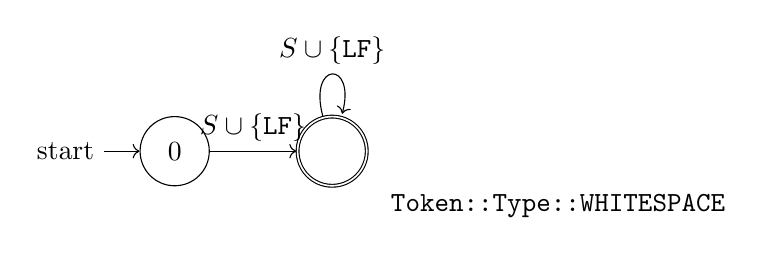
\begin{tikzpicture}
\node[state,initial] (q1) {$0$};
\coordinate[right of=q1] (tq1) {};
\node[state, right of=tq1, accepting] (q2) {};
\node [below right = 0.1cm and 0.3cm of q2]
    {\texttt{Token::Type::WHITESPACE}};
\draw
    (q1) edge[above, ->] node{$S\cup\{\texttt{LF}\}$} (q2)
    (q2) edge[loop above, ->] node{$S\cup\{\texttt{LF}\}$} (q2);
\end{tikzpicture}
\caption{States \& transitions for recognising
whitespace}
\end{figure}

\begin{figure}[H]
\centering
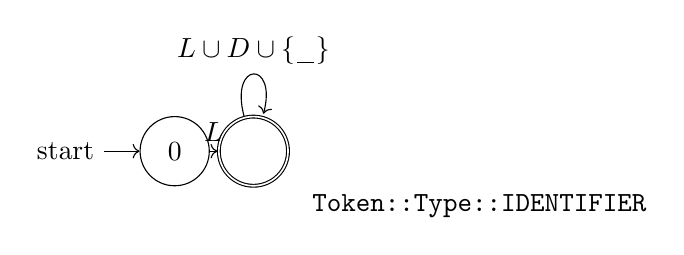
\begin{tikzpicture}
\node[state,initial] (q1) {$0$};
\node[state, right of=q1, accepting] (q2) {};
\node [below right = 0.1cm and 0.3cm of q2]
    {\texttt{Token::Type::IDENTIFIER}};
\draw
    (q1) edge[above, ->] node{$L$} (q2)
    (q2) edge[loop above, ->] node{$L \cup D \cup \{\texttt{\_}\}$} (q2);
\end{tikzpicture}
\caption{States \& transitions for recognising
identifiers/keywords}
\end{figure}

\begin{figure}[H]
\centering
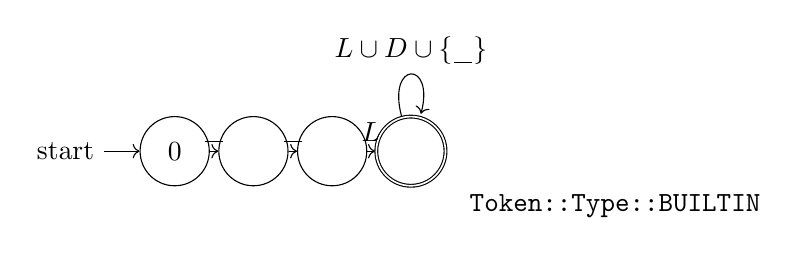
\begin{tikzpicture}
\node[state,initial] (q1) {$0$};
\node[state, right of=q1] (q2) {};
\node[state, right of=q2] (q3) {};
\node[state, right of=q3, accepting] (q4) {};
\node [below right = 0.1cm and 0.3cm of q4]
    {\texttt{Token::Type::BUILTIN}};

\draw
    (q1) edge[above, ->] node{\texttt{\_}} (q2)
    (q2) edge[above, ->] node{\texttt{\_}} (q3)
    (q3) edge[above, ->] node{$L$} (q4)
    (q4) edge[loop above, ->] node{$L \cup D \cup \{\texttt{\_}\}$} (q4);
\end{tikzpicture}
\caption{States \& transitions for recognising
builtins}
\end{figure}


\begin{figure}[H]
\centering
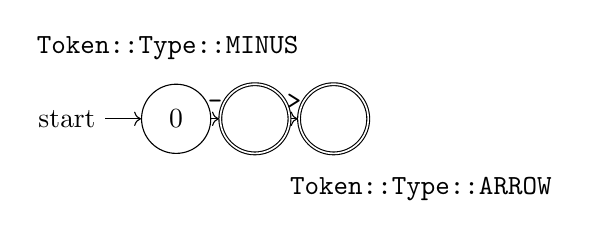
\begin{tikzpicture}
\node[state,initial] (q1) {$0$};
\node[state, right of=q1, accepting] (q2) {};
\node[state, right of=q2, accepting] (q3) {};
\node [above left = 0.3cm and -1cm of q2]
    {\texttt{Token::Type::MINUS}};
\node [below right = 0.3cm and -1cm of q3]
    {\texttt{Token::Type::ARROW}};
\draw
    (q1) edge[above, ->] node{\texttt{-}} (q2)
    (q2) edge[above, ->] node{\texttt{>}} (q3);
\end{tikzpicture}
\caption{States \& transitions for recognising
minus and arrow (\texttt{->})}
\end{figure}

\begin{figure}[H]
\centering
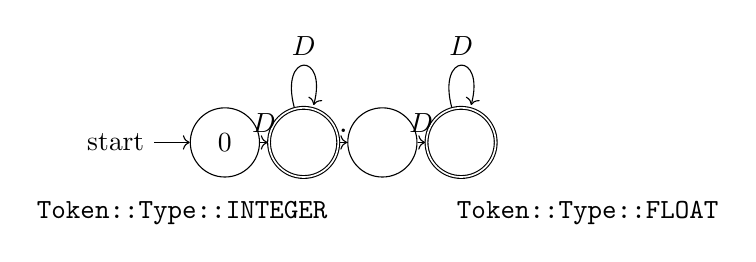
\begin{tikzpicture}
\node[state,initial] (q1) {$0$};
\node[state, right of=q1, accepting] (q2) {};
\node[state, right of=q2] (q3) {};
\node[state, right of=q3, accepting] (q4) {};
\node [below left = 0.3cm and -0.75cm of q2]
    {\texttt{Token::Type::INTEGER}};
\node [below right = 0.3cm and -0.5cm of q4]
    {\texttt{Token::Type::FLOAT}};
\draw
    (q1) edge[above, ->] node{$D$} (q2)
    (q2) edge[loop above, ->] node{$D$} (q2)
    (q2) edge[above, ->] node{\texttt{.}} (q3)
    (q3) edge[above, ->] node{$D$} (q4)
    (q4) edge[loop above, ->] node{$D$} (q4)
    ;
\end{tikzpicture}
\caption{States \& transitions for recognising
integers and floats}
\end{figure}

\begin{figure}[H]
\centering
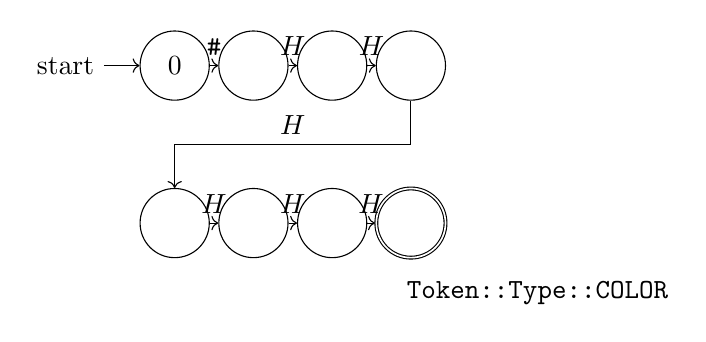
\begin{tikzpicture}
\node[state,initial] (q1) {$0$};
\node[state, right of=q1] (q2) {};
\node[state, right of=q2] (q3) {};
\node[state, right of=q3] (q4) {};

\coordinate[below of=q1] (bq1) {};
\coordinate[below of=q4] (bq4) {};

\node[state, below of=bq1] (q5) {};
\node[state, right of=q5] (q6) {};
\node[state, right of=q6] (q7) {};
\node[state, right of=q7, accepting] (q8) {};
\node [below right = 0.3cm and -0.5cm of q8]
    {\texttt{Token::Type::COLOR}};
\draw
    (q1) edge[above, ->] node{\texttt{\#}} (q2)
    (q2) edge[above, ->] node{$H$} (q3)
    (q3) edge[above, ->] node{$H$} (q4)
    (q4) -- (bq4)
    (bq4) edge[above] node{$H$} (bq1)
    (bq1) edge[->] (q5)
    (q5) edge[above, ->] node{$H$} (q6)
    (q6) edge[above, ->] node{$H$} (q7)
    (q7) edge[above, ->] node{$H$} (q8)
    ;
\end{tikzpicture}
\caption{States \& transitions for recognising
colours}
\end{figure}

\begin{figure}[H]
\centering
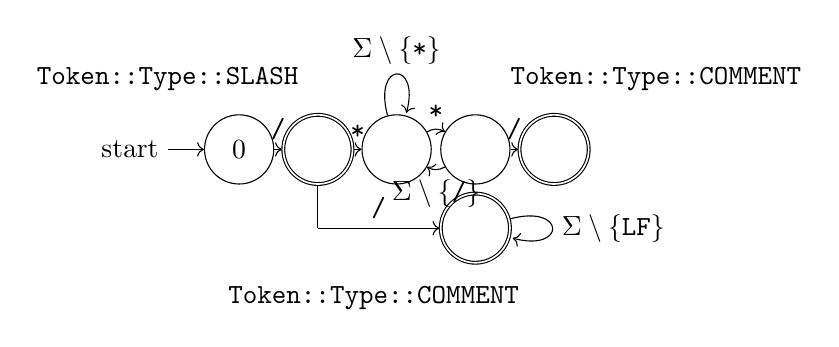
\begin{tikzpicture}
\node[state,initial] (q1) {$0$};
\node[state, right of=q1,accepting] (q2) {};

\coordinate[below of=q2] (bq2) {};

\node[state, right of=q2] (q4) {};
\node[state, right of=q4] (q5) {};
\node[state, right of=q5,accepting] (q6) {};

\node[state, below of=q5, accepting] (q3) {};

\node [above left = 0.3cm and -0.2cm of q2]
    {\texttt{Token::Type::SLASH}};

\node [above right = 0.3cm and -1cm of q6]
    {\texttt{Token::Type::COMMENT}};

\node [below left = 0.3cm and -1cm of q3]
    {\texttt{Token::Type::COMMENT}};

\draw
    (q1) edge[above, ->] node{\texttt{/}} (q2)
    (q2) -- (bq2)
    (bq2) edge[above, ->] node{\texttt{/}} (q3)
    (q3) edge[loop right, ->] node{$\Sigma \setminus \{\texttt{LF}\}$} (q3)
    (q2) edge[above, ->] node{\texttt{*}} (q4)
    (q4) edge[loop above, ->] node{$\Sigma \setminus \{\texttt{*}\}$} (q4)
    (q4) edge[above, bend left, ->] node{\texttt{*}} (q5)
    (q5) edge[below, bend left, ->] node{$\Sigma \setminus \{\texttt{/}\}$} (q4)
    (q5) edge[above, ->] node{\texttt{/}} (q6)
    ;
\end{tikzpicture}
\caption{States \& transitions for recognising
slashes and comments}
\end{figure}

\begin{figure}[H]
\centering
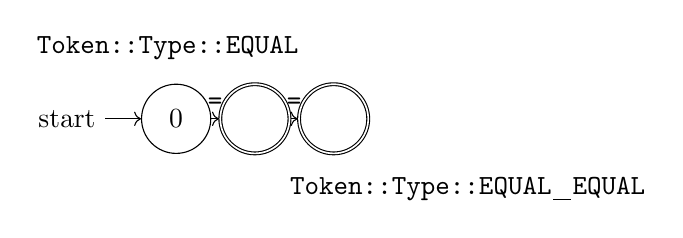
\begin{tikzpicture}
\node[state,initial] (q1) {$0$};
\node[state, right of=q1, accepting] (q2) {};
\node[state, right of=q2, accepting] (q3) {};
\node [above left = 0.3cm and -1cm of q2]
    {\texttt{Token::Type::EQUAL}};
\node [below right = 0.3cm and -1cm of q3]
    {\texttt{Token::Type::EQUAL\_EQUAL}};
\draw
    (q1) edge[above, ->] node{\texttt{=}} (q2)
    (q2) edge[above, ->] node{\texttt{=}} (q3);
\end{tikzpicture}
\caption{States \& transitions for assign
and is equal to}
\end{figure}

\begin{figure}[H]
\centering
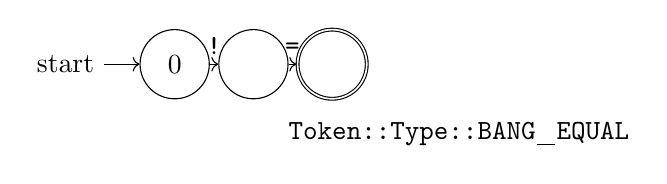
\begin{tikzpicture}
\node[state,initial] (q1) {$0$};
\node[state, right of=q1] (q2) {};
\node[state, right of=q2, accepting] (q3) {};
\node [below right = 0.3cm and -1cm of q3]
    {\texttt{Token::Type::BANG\_EQUAL}};
\draw
    (q1) edge[above, ->] node{\texttt{!}} (q2)
    (q2) edge[above, ->] node{\texttt{=}} (q3);
\end{tikzpicture}
\caption{States \& transitions for not equal to}
\end{figure}


\begin{figure}[H]
\centering
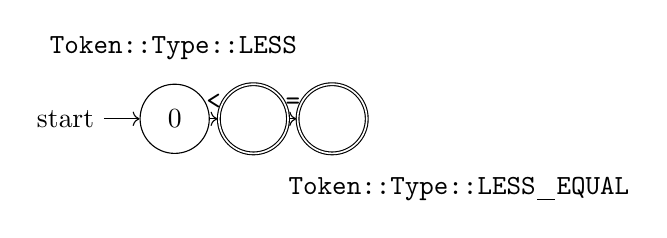
\begin{tikzpicture}
\node[state,initial] (q1) {$0$};
\node[state, right of=q1, accepting] (q2) {};
\node[state, right of=q2, accepting] (q3) {};
\node [above left = 0.3cm and -1cm of q2]
    {\texttt{Token::Type::LESS}};
\node [below right = 0.3cm and -1cm of q3]
    {\texttt{Token::Type::LESS\_EQUAL}};
\draw
    (q1) edge[above, ->] node{\texttt{<}} (q2)
    (q2) edge[above, ->] node{\texttt{=}} (q3);
\end{tikzpicture}
\caption{States \& transitions for less than
and less than or equal to}
\end{figure}

\begin{figure}[H]
\centering
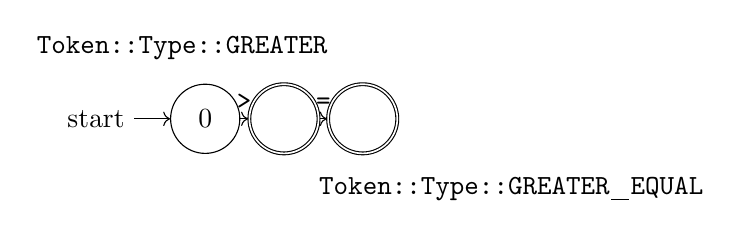
\begin{tikzpicture}
\node[state,initial] (q1) {$0$};
\node[state, right of=q1, accepting] (q2) {};
\node[state, right of=q2, accepting] (q3) {};
\node [above left = 0.3cm and -1cm of q2]
    {\texttt{Token::Type::GREATER}};
\node [below right = 0.3cm and -1cm of q3]
    {\texttt{Token::Type::GREATER\_EQUAL}};
\draw
    (q1) edge[above, ->] node{\texttt{>}} (q2)
    (q2) edge[above, ->] node{\texttt{=}} (q3);
\end{tikzpicture}
\caption{States \& transitions for greater than
and greater than or equal to}
\end{figure}


\begin{figure}[H]
\centering
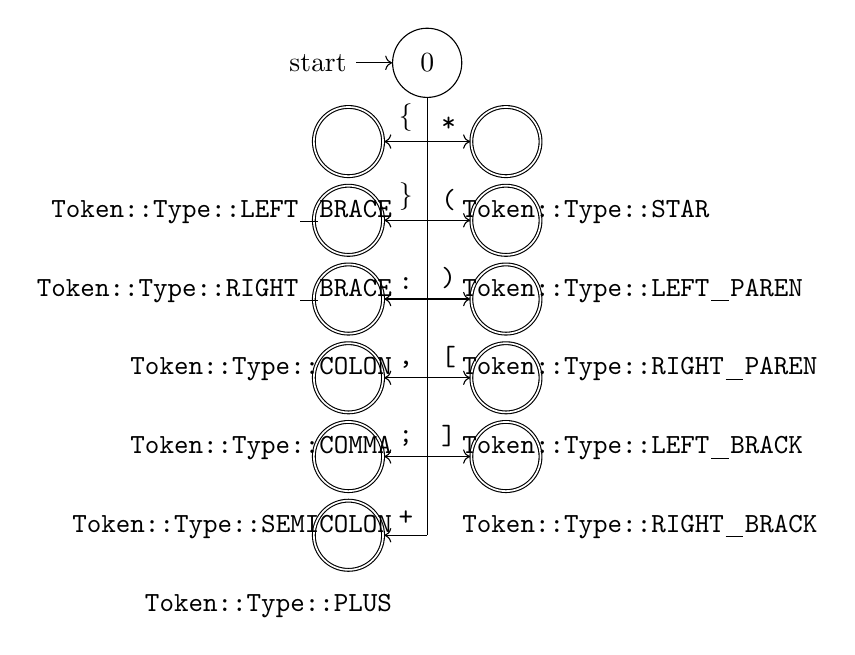
\begin{tikzpicture}
\node[state,initial] (q1) {$0$};

\coordinate[below of=q1] (b1) {};
\coordinate[below of=b1] (b2) {};
\coordinate[below of=b2] (b3) {};
\coordinate[below of=b3] (b4) {};
\coordinate[below of=b4] (b5) {};
\coordinate[below of=b5] (b6) {};

\node[state, right of=b1, accepting] (q2) {};
\node[state, below of=q2, accepting] (q3) {};
\node[state, below of=q3, accepting] (q4) {};
\node[state, below of=q4, accepting] (q5) {};
\node[state, below of=q5, accepting] (q6) {};

\node[state, left of=b1, accepting] (q7) {};
\node[state, below of=q7, accepting] (q8) {};
\node[state, below of=q8, accepting] (q9) {};
\node[state, below of=q9, accepting] (q10) {};
\node[state, below of=q10, accepting] (q11) {};
\node[state, below of=q11, accepting] (q12) {};

\node [below right = 0.3cm and -1cm of q2]
    {\texttt{Token::Type::STAR}};
\node [below right = 0.3cm and -1cm of q3]
    {\texttt{Token::Type::LEFT\_PAREN}};
\node [below right = 0.3cm and -1cm of q4]
    {\texttt{Token::Type::RIGHT\_PAREN}};
\node [below right = 0.3cm and -1cm of q5]
    {\texttt{Token::Type::LEFT\_BRACK}};
\node [below right = 0.3cm and -1cm of q6]
    {\texttt{Token::Type::RIGHT\_BRACK}};

\node [below left = 0.3cm and -1cm of q7]
    {\texttt{Token::Type::LEFT\_BRACE}};
\node [below left = 0.3cm and -1cm of q8]
    {\texttt{Token::Type::RIGHT\_BRACE}};
\node [below left = 0.3cm and -1cm of q9]
    {\texttt{Token::Type::COLON}};
\node [below left = 0.3cm and -1cm of q10]
    {\texttt{Token::Type::COMMA}};
\node [below left = 0.3cm and -1cm of q11]
    {\texttt{Token::Type::SEMICOLON}};
\node [below left = 0.3cm and -1cm of q12]
    {\texttt{Token::Type::PLUS}};

\draw
    (q1) -- (b1)
    (b1) -- (b2)
    (b2) -- (b3)
    (b3) -- (b4)
    (b4) -- (b5)
    (b5) -- (b6)
    ;

\draw
    (b1)  edge[above, ->] node{\texttt{*}} (q2)
    (b2) edge[above, ->] node{\texttt{(}} (q3)
    (b3) edge[above, ->] node{\texttt{)}} (q4)
    (b4) edge[above, ->] node{\texttt{[}} (q5)
    (b5) edge[above, ->] node{\texttt{]}} (q6)

    (b1) edge[above, ->] node{\texttt{\{}} (q7)
    (b2) edge[above, ->] node{\texttt{\}}} (q8)
    (b3) edge[above, ->] node{\texttt{:}} (q9)
    (b4) edge[above, ->] node{\texttt{,}} (q10)
    (b5) edge[above, ->] node{\texttt{;}} (q11)
    (b6) edge[above, ->] node{\texttt{+}} (q12)
    ;
\end{tikzpicture}
\caption{States \& transitions for single letter tokens}
\end{figure}

\subsubsection{The Builder \& Director}

Each sequence of states present is directly
represented in code within the
\texttt{LexerDirector} using methods provided by
the \texttt{LexerBuilder}.

\lstinputlisting[
firstline=297,
lastline=309,
caption={Code specification of
the comments in the \texttt{LexerDirector}
(lexer/LexerDirector.cpp)},
label=lst:commenttransitions
]{lexer/LexerDirector.cpp}

The \texttt{LexerBuilder} keeps track of these
transitions using less efficient data structures
such as hash maps (\texttt{std::unordered\_map})
and sets (\texttt{std::unordered\_set}).

Then the \texttt{build()} method processes the
user defined transitions and normalises everything
into a single transition table for use in a DFSA.
Additionally, it also produces two other
artefacts. The first is called
\texttt{categoryIndexToChecker}. It is a hash map
from the index of a category to a lambda function
which takes a character as input and returns true
or false.

The lambdas and the category indices are also
registered by the user. See \listref{checkerreg}
for a registration example. Additionally, the
category indices although they are integers for
readability they are defined as an enumeration.

\lstinputlisting[
firstline=51,
lastline=58,
caption={Registration of the hexadecimal category
checker (lexer/LexerDirector.cpp)},
label=lst:checkerreg
]{lexer/LexerDirector.cpp}

The second artefact produced by the builder is
also a hash map from final states to their
associated token type.

The transition table is then passed onto the DFSA.
And the DFSA, and the two artefacts are passed
onto the Lexer class.

\lstinputlisting[
firstline=210,
lastline=224,
caption={Constructions of the Lexer
(lexer/LexerBuilder.cpp)},
]{lexer/LexerBuilder.cpp}

\subsubsection{The Actual Lexer}

The lexer's core is as was described during the
lectures and the core/main method is
\texttt{simulateDFSA()}.

It also has a number of very important auxiliary
methods and behavioural changes. Specifically, the
\texttt{updateLocationState()}, see
\listref{updateloc}, is critical for providing
adequate error messages both during the current
stage and for later stages. This function is
called every time a lexeme is consumed allowing
the lexer to keep track of where in the file it
is, in terms of lines and columns.

\lstinputlisting[
firstline=110,
lastline=122,
caption={The \texttt{updateLocationState()} lexer
method (lexer/Lexer.cpp)},
label=lst:updateloc
]{lexer/Lexer.cpp}

Additionally, if an invalid / non-accepting state
is reached the invalid lexeme is consumed and the
user is warned, see \listref{lexererrors}. After
this the lexer, is left in a still operational state.
Hence, \texttt{nextToken()} can be used again.

 This is critical to provide users of the
 \texttt{PArL} compiler with a list of as many
 errors as possible, since it would be a bad
 experience to have to constantly run the
 \texttt{PArL} compiler to see the next error.

\lstinputlisting[
firstline=56,
lastline=84,
caption={Error handling mechanism in the
\texttt{nextToken()} lexer method
(lexer/Lexer.cpp)},
label=lst:lexererrors
]{lexer/Lexer.cpp}

\subsubsection{Hooking up the Lexer to the Runner}

The \texttt{Runner} class is the basic structure
which connects all the stages of the
compiler together together.

In this case the Runner passes in a reference to
the lexer into the parser, this allows the parser
to request tokens and they are computed on demand
improving overall performance. Additionally, this
has the benefit of allowing the parsing of larger
and multiple files since, the parser is no longer
limited by the amount of usable memory, since it
does not need to load the whole file.

However, in this case no such optimisation is
present.

\lstinputlisting[
firstline=22,
lastline=28,
caption={The Runner constructor passes
\texttt{mLexer} into the Parser constructor
(runner/Runner.cpp)}
]{runner/Runner.cpp}

\section{The \texttt{Parser}}

\subsection{Modified EBNF}

\setlength{\grammarparsep}{8pt plus 1pt minus 1pt} % increase separation between rules
\setlength{\grammarindent}{8.5em} % increase separation between LHS/RHS

Some modifications were applied to the original EBNF. These
modifications were motivated by the prospects of an improved
user experience, a more uniform type system and the reduction of
code complexity in later stages.

\begin{center}
\begin{grammar}
<Letter> ::= `A'-`Z' | `a'-`z'

<Digit> ::= `0'-`9'

<Hex> ::= `A'-`F' | `a'-`F' | <Digit>

<Identifier> ::= <Letter> \{`\_' | <Letter> | <Digit>\}

<BooleanLiteral> ::= `true' | `false'

<IntegerLiteral> ::= <Digit> \{<Digit>\}

<FloatLiteral> ::= <Digit> \{<Digit>\} `.' <Digit> \{<Digit>\}

<ColorLiteral> ::= `\#' <Hex> <Hex> <Hex> <Hex> <Hex> <Hex>

<ArrayLiteral> ::= `[' [<Epxr> \{`,' <Epxr>\}] `]'

<PadWidth> ::= `\_\_width'

<PadHeight> ::= `\_\_height'

<PadRead> ::= `\_\_read' <Epxr> `,' <Epxr>

<PadRandomInt> ::= `\_\_random\_int' <Epxr>

<Literal> ::= <BooleanLiteral>
\alt <IntegerLiteral>
\alt <FloatLiteral>
\alt <ColorLiteral>
\alt <ArrayLiteral>
\alt <PadWidth>
\alt <PadHeight>
\alt <PadRead>
\alt <PadRandomInt>

<Type> ::= (`bool' | `int' | `float' | `color') [ `[' <IntegerLiteral> `]' ]

<SubEpxr> ::= `(' <Epxr> `)'

<Variable> ::= <Identifier>

<ArrayAccess> ::= <Identifier> `[' <Epxr> `]'

<FunctionCall> ::= <Identifier> `(' [<Epxr> \{`,' <Epxr>\}] `)'

<Epxr> ::= <LogicOr> [`as' <Type>]

<LogicOr> ::= <LogicAnd> \{`or' <LogicAnd>\}

<LogicAnd> ::= <Equality> \{`and' <Equality>\}

<Equality> ::= <Comparison> \{(`==' | `!=') <Comparison>\}

<Comparison> ::= <Term> \{(`<' | `<=' | `>' | `>=') <Term>\}

<Term> ::= <Factor> \{(`+' | `-') <Factor>\}

<Factor> ::= <Unary> \{(`*' | `/') <Unary>\}

<Unary> ::= (`-' | `not') <Unary> | <Primary>

<RefExpr> ::= <Variable>
\alt <ArrayAccess>
\alt <FunctionCall>

<Primary> ::= <Literal>
\alt <SubExpr>
\alt <RefExpr>

<Program> ::= \{<Stmt>\}

<Stmt> ::= <Block>
\alt <VaribaleDecl> `;'
\alt <FunctionDecl>
\alt <Assignment> `;'
\alt <PrintStmt> `;'
\alt <DelayStmt> `;'
\alt <WriteBoxStmt> `;'
\alt <WriteStmt> `;'
\alt <ClearStmt> `;'
\alt <IfStmt>
\alt <ForStmt>
\alt <WhileStmt>
\alt <ReturnStmt> `;'

<Block> ::= `\{' \{<Stmt>\} `\}'

<VariableDecl> ::= `let' <Identifier> `:' <Type> `='
<Epxr>

<FormalParam> ::= <Identifier> `:' <Type>

<FunctionDecl> ::= `fun' <Identifier> `(' [ <ForamlParam>
\{`,' <FormalParam>\}] `)' `->' <Type> <Block>

<Assignment> ::= <Identifier> [`[' <Epxr> `]'] `='
<Epxr>

<PrintStmt> ::= `\_\_print' <Epxr>

<DelayStmt> ::= `\_\_delay' <Epxr>

<WriteBoxStmt> ::= `\_\_write\_box' <Epxr>`,'
<Epxr>`,'<Epxr>`,' <Epxr>`,'<Epxr>

<WriteStmt> ::= `\_\_write' <Epxr>`,' <Epxr>`,'<Epxr>

<ClearStmt> ::= `\_\_clear' <Epxr>

<IfStmt> ::= `if' `(' <Expr> `)' <Block> [`else' <Block>]

<ForStmt> ::= `for' `(' [<VariableDecl>] `;' <Expr> `;'
[<Assignment>] `)' <Block>

<WhileStmt> ::= `while' `(' <Expr> `)' <Block>

<ReturnStmt> ::= `return' <Expr>
\end{grammar}
\end{center}

\subsubsection{Improved Precedence}\label{sss:improvedprec}

The changes to the EBNF which improve programmer usability are
the additions of a number other expression stages, such as
$\langle$LogicOr$\rangle$, $\langle$LogicAnd$\rangle$, etc. The
main reason for the addition of such rules is to further enforce
a more natural operation precedence. For example, a programmer
often expects that comparison operators such as \texttt{<} and
\texttt{>}, bind tighter than \texttt{and} or \texttt{or}, hence
the compiler needs to make sure that comparison operators are
executed before logical operators. This can be enforced by the
grammar itself hence the changes.

\subsubsection{Better Arrays}\label{sss:secarrays}

The way arrays were being implemented in the original grammar
was very restrictive. Instead an approach for treating arrays as
their own type and literal was taken up.

The $\langle$Type$\rangle$ and $\langle$Literal$\rangle$
productions were augmented to improve array support. This helped
simplify the $\langle$Identifier$\rangle$ (in the original EBNF)
, $\langle$VariableDecl$\rangle$ and
$\langle$FormalParam$\rangle$ productions.

This opens up further support for more complicated types later
on. For example, the $\langle$Type$\rangle$ production can be
further augmented to support more expressive types.

\begin{grammar}

<StructField> ::= <Identifier> `:' <Type>

<Struct> ::= `struct' <Identifier> `\{' \{<StructField> `;'\} `\}'

<TypeDecl> ::= <Struct>

<Base> ::= (`bool' | `int' | `float' | `color')

<Array> ::= <Type> `[' <IntegerLiteral> `]'

<Pointer> ::= <Type> `*'

<Type> ::= <Identifier>
\alt <Base>
\alt <Array>
\alt <Pointer>
\end{grammar}

\begin{note}
The $\langle$ForamlParam$\rangle$ is indeed being repeated in a
number of places. However, this is not really a problem. When it
comes to specifications, repetition which improves clarity is
``good'' repetition.
\end{note}

\label{sss:primitive}Additionally, some of the ground work for
these improvements has already been laid out in the internal
type system (see \listref{internaltypesystem} and
\listref{primitive}).

\lstinputlisting[
linerange={185-197}, caption={Mechanism for internally storing
types within the compiler (parl/Core.hpp).},
label=lst:internaltypesystem
]{parl/Core.hpp}

\begin{lstlisting}[caption={The \texttt{Primitive} class
declaration (parl/Core.hpp).}, label=lst:primitive]
struct Primitive {
    template <typename T>
    [[nodiscard]] bool is() const {
        return std::holds_alternative<T>(data);
    }

    template <typename T>
    [[nodiscard]] const T &as() const {
        return std::get<T>(data);
    }

    ...

    bool operator!=(Primitive const &other) {
        return !operator==(other);
    }

    std::variant<std::monostate, Base, Array> data{};
};
\end{lstlisting}

The \texttt{box} type is a special type of pointer
object which has value semantics that is it behaves
as though it were the object it contains.

This is critical because self-referential types like
$\langle$Array$\rangle$ are not easily representable within
\CC{} since, something like \listref{unboundedsize}, is not
allowed.

\begin{lstlisting}[caption={An size unbounded type in \CC{}
(parl/Core.hpp).}, label=lst:unboundedsize]
struct SelfRef;

struct Container {
    Other other;
    SelfRef ref;
};

struct Primitive {
    std::variant<std::monostate, Container> data{};
};
\end{lstlisting}

This is because the \CC{} compiler is incapable of determining
the size of said type at compile-time. Hence, a pointer for said
type is required. And the pointer wrapper \texttt{box<>} allows
it to be copied as tough it were a value.

\begin{attrib}
    \textcolor{UMRed}{Jonathan Müller} presented the
    \texttt{box<>} type in a discussion regarding the exact same
    issue, on his
    \href{https://www.foonathan.net/2022/05/recursive-variant-box/}{
    blog}, \texttt{foonathan}.
\end{attrib}

These changes to type also require additional changes to how
variables are referenced in expressions, hence why
$\langle$RefExpr$\rangle$ was added.

\begin{todo}
Due to $\langle$RefExpr$\rangle$ more complicated referencing
such as `\texttt{object.something}' (\texttt{struct} member
referencing) should be possible.
\end{todo}

Finally, the $\langle$ArrayLiteral$\rangle$ has been improved to
support expressions instead of just only literals.

\subsubsection{Removing Eye-Candy}\label{eyecandy}

Adding this system however, would significantly increases the
complexity of semantic analysis, if the proposed syntax sugar
for arrays is kept.

Because of this the following two conveniences \texttt{let a:
int[] = [1,1,1];} and \texttt{let a: int[3] = [1];} have been
dropped, from the language.

This is because such syntax not only complicates the grammar but
it also significantly increases the complexity of semantic
analysis.

The best way to handle such syntax is to have a de-sugaring \&
type inference sub-phase before type checking, ensure proper
separation of concerns.

\subsection{Parsing \& The Abstract Syntax Tree (AST)}

The AST is the data structure which is produced by the
\texttt{Parser}. The nodes of the AST are \emph{almost} a
one-to-one representation of the productions in the grammar (see
\listref{funccallast}).

\lstinputlisting[linerange={129-136}, caption={The
\texttt{FunctionCall} AST node class (parl/AST.hpp).},
label=lst:funccallast ]{parl/AST.hpp}

The only significant difference in these nodes is the
\texttt{position} field. This gets populated by the parser using
the location of a token in the original source file. This is
again critical for adequate error messaging in later stages.

\pagebreak

\lstinputlisting[
linerange={146-154}, caption={The \texttt{Binary} AST node class
(parl/AST.hpp).}, label=lst:binaryast ]{parl/AST.hpp}

\lstinputlisting[
linerange={156-163}, caption={The \texttt{Unary} AST node class
(parl/AST.hpp).}, label=lst:unaryast ]{parl/AST.hpp}

Apart from \texttt{position} field the only other difference is
the usage of a \texttt{Binary} and \texttt{Unary} node (see
\listref{binaryast} and \listref{unaryast}), instead of a node
for each type of the expression types $\langle$LogicOr$\rangle$,
etc. grammar rules discussed in \ref{sss:improvedprec}. This is
because those productions enforce precedence, and precedence,
within an AST is not controlled by the nodes but by the
structure of the AST itself.

Additionally, a number of the nodes override the
\texttt{accept()} method specified by the pure virtual class
\texttt{Node}. This is the basis for the visitor pattern which
apart form the parser is the backbone of the later stages.

\subsection{The Actual \texttt{Parser}}

The \texttt{Parser} can be split into these four main sections.

\begin{itemize}
    \item AST Generation;
    \item Token Buffering;
    \item Token Matching;
    \item and, Error Handling/Recovery.
\end{itemize}

\subsubsection{Token Buffering}

The \texttt{Parser} of course requires access to the tokens
generated from the source file. However, sometimes the
\texttt{Parser} might require more than token to decide. This is
quite easy to implement if the \texttt{Parser} has available to
it, at initialisation, all the tokens.

However, as described in \ref{sss:runnerlexer}, This is not the
case. The \texttt{Parser} requests token on demand from
\texttt{Lexer}. This of course means that the machinery for
handling tokens is a bit more complicated as it needs to cater
for lookahead.

To solve this issue a window-based approach was adopted. The
\texttt{Parser} has a moving buffer/window called
\texttt{mTokenBuffer}, whose size is specified at compile-time
using a C-style macro `\texttt{\#define LOOKAHEAD (2)}'. The
core methods for this aspect of the parser are
\texttt{moveWindow()} and \texttt{nextToken()} (see
\listref{tokenmovewindow} and \listref{tokennexttoken}).

\lstinputlisting[linerange={1111-1119}, caption={The
\texttt{moveWindow()} \texttt{Parser} methods
(parser/Parser.cpp).},
label=lst:tokenmovewindow]{parser/Parser.cpp}

\pagebreak

\lstinputlisting[linerange={1121-1131}, caption={The
\texttt{nextToken()} \texttt{Parser} methods
(parser/Parser.cpp).},
label=lst:tokennexttoken]{parser/Parser.cpp}

\begin{note}
Within the \texttt{nextToken()} method whitespace and comments
are being explicitly ignored.
\end{note}

\begin{todo}
Comments can be integrated into the AST. This would allows
printing or formatting visitors to properly format code whilst
still preserving any comments.
\end{todo}

\subsubsection{Token Matching}

The previous methods all facilitate the more important token
matching methods which are:

\begin{itemize}
    \item \texttt{peek()};
    \item \texttt{advance()};
    \item \texttt{previous()};
    \item \texttt{isAtEnd()};
    \item \texttt{peekMatch()};
    \item \texttt{match()};
    \item and, \texttt{consume()}.
\end{itemize}

Arguably, the most important of these methods is
\texttt{consume()}. It takes in a token type and an error
message, which it uses to warn the user if the specified token
type is not matched (see \listref{consume}).

\begin{lstlisting}[caption={The \texttt{consume()} Parser method
(parser/Parser.hpp).},
label=lst:consume]
template <typename... T>
void consume(
    Token::Type type,
    fmt::format_string<T...> fmt,
    T&&... args
) {
    if (check(type)) {
        advance();
    } else {
        error(fmt, args...);
    }
}
\end{lstlisting}

The main reason for templating such a method is to provide an
easy interface for formattable strings using
\href{https://github.com/fmtlib/fmt}{fmtlib}. The main feature
this library provides is the ability to specify placeholders in
the string itself using `\texttt{\{\}}'. Usage of this
functionality is demonstrated in the AST generator methods (see
\listref{consumeusage}).

\begin{lstlisting}[caption={Usage of the \texttt{consume()}
method in the \texttt{formalParam()} generator method
(parser/Parser.cpp).}, label=lst:consumeusage]
std::unique_ptr<core::FormalParam> Parser::formalParam() {
    consume(
        Token::Type::IDENTIFIER,
        "expected identifier token "
        "instead received {}",
        peek().toString()
    );

    ...
\end{lstlisting}


The \texttt{peekMatch()} method is a simple method which returns
true if at least one of the provided token types match. An
example demonstrating the usage of \texttt{peekMatch()} is the
$\langle$Comparison$\rangle$ production, since there are four
token types which match. The \texttt{match()} method is a simple
extension of \texttt{peekMatch()} which consumes the token if it
matches.

The methods \texttt{advance()}, \texttt{previous()} and
\texttt{isAtEnd()} are quite self explanatory.
\texttt{advance()} moves the buffer window one step forward,
\texttt{previous()} returns the last consumed token, and
\texttt{isAtEnd()} checks whether or not the \texttt{Parser} has
reached an `End of File' token.

\texttt{peek()} is also very simple it allows the
\texttt{Parser} to see the token without consuming it. However,
since the \texttt{Parser} might need to lookahead
\texttt{peek()} supports an offset. Because of this calls to
\texttt{peek()} have to be checked to ensure valid access (see
\listref{peek}). This is done using the \texttt{abort\_if()}
function which prints an error message and aborts the program.
This is very similar to a \texttt{static\_assert} however, it is
performed at runtime (see \listref{abortif}).

\lstinputlisting[linerange={1137-1145}, caption={The
\texttt{peek()} \texttt{Parser} method (parser/Parser.cpp).},
label=lst:peek]{parser/Parser.cpp}

\lstinputlisting[linerange={13-41}, caption={The abort
functionality present in the codebase (parl/Core.hpp).},
label=lst:abortif]{parl/Core.hpp}

\begin{note}
Since the usage of \texttt{abort()} and \texttt{abort\_if()} is
internal to the code, it only makes sense for these functions to
be enabled during debug builds only. Hence, the implementations
are enclosed between an \texttt{\#ifdef, \#else, \#endif} macro.
When \texttt{NDEBUG}, which stand for no-debug, is defined the
function bodies are hollowed out allowing the \CC{} compiler to
optimise them out.
\end{note}

\subsubsection{Error Handling/Synchronization}

Error handling and synchronization is a critical part of the
\texttt{Parser}. With regards to developer productivity, having
meaningful errors is extremely valuable. But apart from that
being able see all the errors in a file is also crucial. This
means that a developer will waste less time re-running the
compiler to find all the errors present in the source code.

\begin{attrib}
This processes is referred to as
\href{https://craftinginterpreters.com/parsing-expressions.html#synchronizing-a-recursive-descent-parser}{Synchronization}
by the author of
\href{https://craftinginterpreters.com/}{Crafting Interpreters},
\textcolor{UMRed}{Robert Nystrom}.
\end{attrib}

The method for synchronisation in the \texttt{PArL} compiler was
inspired by the above credited author and his usage of
\texttt{Exceptions} as an unrolling primitive. Although
unorthodox, it is very simple way to implement synchronisation.

\pagebreak

\begin{lstlisting}[caption={The \texttt{SyncParser} exception
and the \texttt{error()} method which kick-starts the
synchronisation process (parser/Parser.hpp).},
label=lst:synckickstart]
class SyncParser : public std::exception {};

...

template <typename... T>
void error(fmt::format_string<T...> fmt, T&&... args) {
    mHasError = true;

    Token violatingToken = peek();

    fmt::println(
        stderr,
        "parsing error at {}:{}:: {}",
        violatingToken.getPosition().row(),
        violatingToken.getPosition().col(),
        fmt::format(fmt, args...)
    );

    throw SyncParser{};
}
\end{lstlisting}

However, there is of course a major downside to this. Where
synchronisation happens will affect other error messages which
are reported down stream. This of course has the possibility of
producing false positives. However, in this case error handling
is only best-effort and therefore the possibility of false
positives is accepted. The basic process of synchronising is
consuming as many tokens as possible until the \texttt{Parser}
reaches a token which it believes to be a good restarting point
(see \listref{sync}).

\lstinputlisting[linerange={1195-1243}, caption={The
\texttt{synchronize()} method in the \texttt{Parser} class
(parser/Parser.cpp).}, label=lst:sync]{parser/Parser.cpp}

Finally, the most natural choice for capturing
\texttt{SyncParser} is in the AST generator methods responsible
for generating statements, those being \texttt{program()} and
\texttt{block()}.

\subsubsection{AST Generator Methods}

Finally, the bulk of the parser is actually the generator
methods which build the AST. These methods are not that
complicated and they follow the specified grammar faithfully.

See, \listref{ifstmt} for an example of such a method and see
\listref{methodslist} for a full list of generator methods.

\lstinputlisting[linerange={416-450}, caption={The
\texttt{ifStmt()} node generator method in the \texttt{Parser}
class (parser/Parser.cpp).},
label=lst:ifstmt]{parser/Parser.cpp}

\begin{lstlisting}[caption={The main body of methods in the
\texttt{Parser} class (parser/Parser.hpp).},
label=lst:methodslist]
std::unique_ptr<core::Type> type();

std::unique_ptr<core::Program> program();
std::unique_ptr<core::Stmt> statement();
std::unique_ptr<core::Block> block();
std::unique_ptr<core::VariableDecl> variableDecl();
std::unique_ptr<core::Assignment> assignment();
std::unique_ptr<core::PrintStmt> printStatement();
std::unique_ptr<core::DelayStmt> delayStatement();
std::unique_ptr<core::WriteBoxStmt> writeBoxStatement();
std::unique_ptr<core::WriteStmt> writeStatement();
std::unique_ptr<core::ClearStmt> clearStatement();
std::unique_ptr<core::IfStmt> ifStmt();
std::unique_ptr<core::ForStmt> forStmt();
std::unique_ptr<core::WhileStmt> whileStmt();
std::unique_ptr<core::ReturnStmt> returnStmt();
std::unique_ptr<core::FunctionDecl> functionDecl();
std::unique_ptr<core::FormalParam> formalParam();

std::unique_ptr<core::PadWidth> padWidth();
std::unique_ptr<core::PadHeight> padHeight();
std::unique_ptr<core::PadRead> padRead();
std::unique_ptr<core::PadRandomInt> padRandomInt();
std::unique_ptr<core::BooleanLiteral> booleanLiteral();
std::unique_ptr<core::ColorLiteral> colorLiteral();
std::unique_ptr<core::FloatLiteral> floatLiteral();
std::unique_ptr<core::IntegerLiteral> integerLiteral();
std::unique_ptr<core::ArrayLiteral> arrayLiteral();
std::unique_ptr<core::SubExpr> subExpr();
std::unique_ptr<core::Variable> variable();
std::unique_ptr<core::ArrayAccess> arrayAccess();
std::unique_ptr<core::FunctionCall> functionCall();

std::unique_ptr<core::Expr> expr();
std::unique_ptr<core::Expr> logicOr();
std::unique_ptr<core::Expr> logicAnd();
std::unique_ptr<core::Expr> equality();
std::unique_ptr<core::Expr> comparison();
std::unique_ptr<core::Expr> term();
std::unique_ptr<core::Expr> factor();
std::unique_ptr<core::Expr> unary();
std::unique_ptr<core::Expr> primary();
\end{lstlisting}

\subsection{Pretty Printing}

\subsubsection{Using \texttt{Parser} in the \texttt{Runner}}

The \texttt{Parser} is used in the \texttt{Runner} and assuming
that the parser does not encounter any errors and the
\texttt{mParserDbg} flag is set it can be used to print the AST
using a \texttt{PrinterVisitor}.

\lstinputlisting[linerange={117-127}, caption={The parse segment
of the \texttt{run()} method in the Runner class
(runner/Runner.cpp).}]{runner/Runner.cpp}

Calling the produced \texttt{PArL} binary with the \texttt{-p}
flag will set the \texttt{mParserDbg}, see \figref{test9} and
\figref{parseeg}.

\begin{figure}[H]
\centering
\includegraphics[width=\linewidth]{test9.png}
\caption{\texttt{cat} of the test9.parl.}
\label{fig:test9}
\end{figure}

\begin{figure}[H]
\centering
\includegraphics[height=3.5in]{printervisitoreg.png}
\caption{The AST generated by the syntactically correct program
in testing/test9.parl.}
\label{fig:parseeg}
\end{figure}

\lstinputlisting[linerange={104-110}, caption={The
\texttt{debugParsing()} method in the \texttt{Runner} class
(runner/Runner.cpp).},label=lst:debugparsing]{runner/Runner.cpp}

The \texttt{PrinterVisitor} used in \listref{debugparsing} is
a specialization of the pure virtual \texttt{Visitor} class
in parl/Visitor.hpp.

\begin{lstlisting}[caption={A segment of the pure virtual
\texttt{Visitor} class (parl/Visitor.hpp).},
label=lst:genericvisitor]
...

struct ClearStmt;
struct Block;
struct FormalParam;
struct FunctionDecl;
struct IfStmt;
struct ForStmt;
struct WhileStmt;
struct ReturnStmt;
struct Program;

class Visitor {
   public:
    virtual void visit(Type*) = 0;
    virtual void visit(Expr*) = 0;
    virtual void visit(PadWidth*) = 0;
    virtual void visit(PadHeight*) = 0;
    virtual void visit(PadRead*) = 0;
    virtual void visit(PadRandomInt*) = 0;
    virtual void visit(BooleanLiteral*) = 0;
    virtual void visit(IntegerLiteral*) = 0;
    virtual void visit(FloatLiteral*) = 0;

...
\end{lstlisting}

Due to the way \CC{} handles symbols, the classes which the
visitor can visit must be forward declared manually (see
\listref{genericvisitor}). If no such forward declaration is
made, the compiler will complain about the \texttt{Visitor} and
the \texttt{AST} classes being cyclically dependent.

Additionally, any inheriting visitor such as the
\texttt{PrinterVisitor} can hold state. In fact, this is where
the true power of visitors arises. Being able to hold state
means that complex computations can be carried out on the AST.
For example the \texttt{PrinterVisitor} although simple makes
use of a single variable \texttt{mTabCount} (see
\listref{printnode}), which it uses to affect how much
indentation should be used in printing, allowing us to visualise
the AST.

\lstinputlisting[linerange={45-53}, caption={The
\texttt{visit(core::PadRead *)} method in the
\texttt{PrinterVisitor}
(parser/PrinterVisitor.cpp).},label=lst:printnode]{parser/PrinterVisitor.cpp}

\section{Semantic Analysis}

\subsection{Phases \& Design}

As described in \ref{eyecandy} the Semantic Analysis phase
should be split into a number of sub-phases specifically: symbol
resolution, de-sugaring/type inference and type checking.

However, these steps can be combined together into a single step
phase. There a benefits and downsides to both approaches. The
main benefit of using the first approach is a reduction in
algorithmic complexity. The logic can be separated into
different phases with ease and information from one phase can be
propagated to another. The downside of this approach is that it
actually adds more code for maintenance, since each individual
sub-phase will probably need to be implemented as its own
visitor. The other down side is error management. If an error
occurs in a particular phase since said phase is completely
disjoint from the phases after it a mechanism for propagation
needs to be devised which again further increases complexity. Of
course by the very nature of this argument the monolithic
approach does not suffer for the issues that the sub-phases
approach has. However, it significantly increases complexity
since all sub-phases are being done in a single phase. The other
more glaring issue is the fact that it is much more difficult to
resolve symbols before-hand.

You would want to do so to allow for the location of function
declarations in code to not effect resolution, that is, a
function can be called before it is referenced.

Unfortunately, due to the fact that compiler development was an
organic process and not too much time was spend on deliberation
the semantic analysis phase became monolithic, and hence it
suffers from the issues described above. Of course, this means
location agnostic function declaration are currently \emph{not}
supported by the compiler.

\subsection{The Environment Tree}

Some terminology is required to properly describe the number of
structures which will be used in this section. The following
terms are critical and need to be differentiated properly:

\begin{itemize}
    \item \texttt{SymbolTable}
    \item \texttt{SymbolTableStack}
    \item \texttt{Environment}
    \item \texttt{EnvStack}
    \item \texttt{RefStack}
\end{itemize}

During semantic analysis there is a need for specific data
structures which facilitate scoping rules, type checking, etc.

The most basic data structure which achieves this, is a single
\texttt{SymbolTable}. A symbol table in its simplest form is a
wrapper around a hash map, whose keys are identifiers and values
are \texttt{Symbol}s or any structure which is capable of
storing variable and function signatures.

This approach is quite limiting since it restricts developers
and user of the language to a single global scope. Therefore,
this is structure is not a sufficient solution for most
toy-languages let alone production ready languages.

A better solution is using a stack of symbol tables. This allows
symbol tables to shadow each other allowing for the reuse of
identifiers. Additionally, this further opens up the possibility
of implementing modules at the language-level. The likelihood
that names will be reused across different modules is quite high
and being able to scope modules so they do not interfere with
global scope and each other is necessary for any sufficiently
large project.

\begin{figure}[H]
\centering
\begin{mdframed}[backgroundcolor=UMPaleRed]
\includegraphics[width=\linewidth]{scopedcode.pdf}
\end{mdframed}
\caption{A \texttt{PArL} function with annotated scopes}
\label{fig:scopeannotatedcode}
\end{figure}

The basic premise of using a symbol table stack is described in
\algref{basicsymboltablestack} and \figref{graphicaldecpiction}.
A new symbol table, also referred to as a scope, is pushed onto
a stack only for specific types of AST nodes. The node is then
processed, were ``processing'' often times means considering all
the sub-children of the node, and when processing terminates the
scope is popped. In the context of a purely stack based
implementation this implies that, scopes are only temporary that
is they are lost after being popped.

\begin{algorithm}[H]
\KwData{$N$ the AST node, $S$ the symbol table stack}

\Begin{
    \If{$N$ opens a scope}{
        PushScope($S$)\;
    }
    ProcessNode($N$)\;
    \If{$N$ opens a scope}{
        PopScope($S$)\;
    }
}

\caption{Basic description of \texttt{SymbolTableStack} usage}
\label{alg:basicsymboltablestack}
\end{algorithm}

\begin{figure}[H]
\centering
\begin{mdframed}[backgroundcolor=UMPaleRed]
\includegraphics[width=\linewidth]{symboltablestack.pdf}
\end{mdframed}
\caption{Behaviour of the \texttt{SymbolTableStack} when
considering the code in \figref{scopeannotatedcode}}
\label{fig:graphicaldecpiction}
\end{figure}

The main advantage of using this approach is that the
worst case memory usage is $O(DI)$ where $D$ is the length of a
longest chain of open scopes and $I$ is the size of largest
number of variable declarations within a scope.

However, due to the temporary nature of this approach it does
not lend itself well to a multi-phase approach. This is because
at each phase \texttt{SymbolTable}s have to be regenerated
increase the complexity of each individual phase.

Instead a different approach shall be used. This approach uses
an
\href{https://craftinginterpreters.com/statements-and-state.html#nesting-and-shadowing}{Environment
Tree} and it has also been inspired by
\href{https://craftinginterpreters.com/}{Crafting Interpreters}.

The notion of an \texttt{Environment} is essentially, the same
as a \texttt{SymbolTable}. The only significant change is the
addition of vector of unique pointers to other environments, see
\listref{envclass}.

\begin{lstlisting}[escapechar=!,caption={The
\texttt{Environment} class with \texttt{mChildren} highlighted
(backend/Environment.hpp)}, label=lst:envclass]
class Environment {
   public:
    enum class Type {
        GLOBAL,
        IF,
        ELSE,
        FOR,
        WHILE,
        FUNCTION,
        BLOCK
    };

    void addSymbol(
        std::string const& identifier,
        Symbol const& Symbol
    );
    [[nodiscard]] std::optional<Symbol> findSymbol(
        std::string const& identifier
    ) const;
    Symbol& getSymbolAsRef(std::string const& identifier);

    [[nodiscard]] Environment* getEnclosing() const;
    void setEnclosing(Environment* enclosing);

    [[nodiscard]] Type getType() const;
    void setType(Type type);

    [[nodiscard]] std::optional<std::string> getName(
    ) const;
    void setName(const std::string& name);

    std::vector<std::unique_ptr<Environment>>& children();

    [[nodiscard]] bool isGlobal() const;

    [[nodiscard]] size_t getIdx() const;
    void incIdx();
    void incIdx(size_t inc);

    [[nodiscard]] size_t getSize() const;
    void setSize(size_t size);

   private:
    std::unordered_map<std::string, Symbol> mMap{};
    Type mType{Type::GLOBAL};
    std::optional<std::string> mName{};
    Environment* mEnclosing{nullptr};
    !\colorbox{UMPaleRed}{std::vector<std::unique_ptr<Environment>> mChildren\{\};}!
    size_t mSize{0};
    size_t mIdx{0};
};
\end{lstlisting}

The additional fields present in the \texttt{Environment} class
are there to cater for the needs of each of the phases.

Specifically, \texttt{mType} and \texttt{mName} are used during
semantic analysis and \texttt{mSize} and \texttt{mIdx} are used
during code generation.

Additionally, it is preferable if the interface with which the
phases interact with the \texttt{Environment} tree is identical
to that of a \texttt{SymbolTableStack}, that is the same
\texttt{push()} and \texttt{pop()} methods are used.

Now to facilitate this another two classes need to be defined
\texttt{EnvStack} and \texttt{RefStack}. The main difference
between \texttt{EnvStack} and \texttt{RefStack} is that the
purpose of \texttt{EnvStack} is to construct the
\texttt{Environment} tree whilst \texttt{RefStack} traverses the
environment tree. Due to this \texttt{RefStack} is only required
during the symbol resolution. However, in current implementation
since symbol resolution is combined with type checking, the
Environment tree is generated at the same time as it is being
type checked.

Additionally, in both an \texttt{EnvStack} and a
\texttt{RefStack}, the creation and traversal of the Environment
tree are managed via the \texttt{push()} and \texttt{pop()}
methods.

In an \texttt{EnvStack} \texttt{push()} works by creating a new
environment, setting the enclosing environment to the current
environment and changing the current environment to to the new
environment, see \listref{evnstackpush}. \texttt{pop()} makes
use of the \texttt{mEnclosing} field in the current environment
and just sets the current environment to the enclosing
environment essentially moving up an environment, see
\listref{popenvstack}.

\lstinputlisting[linerange={12-22}, caption={The
\texttt{pushEnv()} method in the \texttt{EnvStack} class
(analysis/EnvStack.cpp)}, label=lst:envstackpush
]{analysis/EnvStack.cpp}

\lstinputlisting[linerange={24-28}, caption={The
\texttt{popEnv()} method in the \texttt{EnvStack} class
(analysis/EnvStack.cpp)}, label=lst:envstackpop
]{analysis/EnvStack.cpp}

The implementations in \texttt{RefStack} are however a bit more
involved. This is because the program has to be able to perform
a step-wise left-first depth-first traversal. The best way
to do this is to make use of a stack and the algorithms
in \listref{refpush} and \listref{refpop}.

\lstinputlisting[linerange={7-17}, caption={The
\texttt{pushEnv()} method in the \texttt{RefStack} class
(ir\_gen/RefStack.cpp)}, label=lst:refpush
]{ir\_gen/RefStack.cpp}

\lstinputlisting[linerange={37-43}, caption={The
\texttt{popEnv()} method in the \texttt{RefStack} class
(ir\_gen/RefStack.cpp)}, label=lst:refpop
]{ir\_gen/RefStack.cpp}

See \figref{refstackdryrun}, for the initial segments of a
traversal. The important thing to note here is that the
correctness of the traversal entirely depends on the usage of
\texttt{push()} and \texttt{pop()}. If used incorrectly the
traversal might be incorrect or the program might crash. Of
course, this is only an implementation detail that is if used
correctly by the compiler developer no such issue should occur.

\begin{figure}[H]
\centering
\begin{mdframed}[backgroundcolor=UMPaleRed]
\includegraphics[width=\linewidth]{refstackdryrun.pdf}
\end{mdframed}
\caption{The initial steps of a traversal performed by
\texttt{RefStack}}
\label{fig:refstackdryrun}
\end{figure}

\subsection{Semantic Analysis}

Having the necessary data structures in place the discussion
will now revolve around Semantic Analysis i.e. the process of
making sure the meaning of the program is correct.

There are four main areas of interest which shall be discussed:
the symbol type, symbol registration/search, type checking and a
unique subset of type checking, return value type verification.

\subsection{The \texttt{Symbol} Type}

Within \texttt{PArL}

This minor change removes the need to throw away Environments
and they can be passed on from one phase to another.

\begin{figure}[H]
\centering
\begin{mdframed}[backgroundcolor=UMPaleRed]
\includegraphics[width=\linewidth]{scopedcode2.pdf}
\end{mdframed}
\caption{Construction of an \texttt{Environment} tree}
\label{fig:scopedcode2}
\end{figure}

The Environment tree is a data structure

\begin{itemize}
    \item Describe Symbol Table.
    \item Describe each element of the symbol table.
    \item Describe the tree approach.
    \item attribute the tree approach to Robert Nystrom as well.
    \item describe the main advantage/disadvantage of using a environment
        approach.
    \item describe the main advantage/disadvantage of using a symbol stack
        approach.
\end{itemize}


\section{Attributions}

\begin{itemize}
    \item Sandro Spina for the brilliant description of table-driven lexers
    \item Robert Nystrom and his great book Crafting Intepreters for a great
        outline for parsing and error recovery/management for languages
        which support exceptions
\end{itemize}


\end{document}
